\documentclass{report}
\usepackage{titlesec}
\titleformat{\chapter}{\normalfont\huge}{\thechapter.}{20pt}{\huge}
\usepackage{tikz}
\usetikzlibrary{shapes.geometric, arrows}
\usepackage{float}
\usepackage[utf8]{inputenc} % Required for inputting international characters
\usepackage[T1]{fontenc} % Output font encoding for international characters
\usepackage{fouriernc} % Use the New Century Schoolbook font
\usepackage{multirow}
\usepackage{relsize}
\usepackage{listings}

\begin{document}
\begin{titlepage} % Suppresses headers and footers on the title page

	\centering % Centre everything on the title page
	
	\scshape % Use small caps for all text on the title page
	
	\vspace*{\baselineskip} % White space at the top of the page
	
	%------------------------------------------------
	%	Title
	%------------------------------------------------
	
	\rule{\textwidth}{1.6pt}\vspace*{-\baselineskip}\vspace*{2pt} % Thick horizontal rule
	\rule{\textwidth}{0.4pt} % Thin horizontal rule
	
	\vspace{1.5\baselineskip} % Whitespace above the title
	
	{\LARGE NON INVASIVE \\\vspace{5.0pt}INFANT SLEEP APNEA DETECTION \\ \vspace{15.0pt} IMPLEMENTATION GUIDE} % Title
	
	\vspace{1.5\baselineskip} % Whitespace below the title
	
	\rule{\textwidth}{0.4pt}\vspace*{-\baselineskip}\vspace{3.2pt} % Thin horizontal rule
	\rule{\textwidth}{1.6pt} % Thick horizontal rule
	
	\vspace{2cm} % Whitespace after the title block
	
	%------------------------------------------------
	%	Subtitle
	%------------------------------------------------
	
	CO321 CO324 CO325 Unified Project % Subtitle or further description
	
	\vspace*{6cm} % Whitespace under the subtitle
	
	%------------------------------------------------
	%	Editor(s)
	%------------------------------------------------
	
	Team
	
	\vspace{0.5\baselineskip} % Whitespace before the editors
	
	{\scshape\Large \begin{tabular}{c l}
	     E/14/158: &Gihan Jayatilaka\\E/14/339: &Suren Sritharan\\E/14/379:& Harshana Weligampola\\E/14/237: &Pankayaraj Pathmanathan\\
	\end{tabular} } % Editor list
	
	\vspace{0.5\baselineskip} % Whitespace below the editor list
	
	\textit{Deaprtment of Computer Engineering \\ Unviersity of Peradeniya} % Editor affiliation
	
	\vfill % Whitespace between editor names and publisher logo
	
	%------------------------------------------------
	%	Publisher
	%------------------------------------------------
	
	
	\vspace{0.3\baselineskip} % Whitespace under the publisher logo
	
	2018 % Publication year
	
\end{titlepage}


\clearpage
\tableofcontents
\clearpage

\chapter{Introduction}

This document gives a step by step guide to implement and develop the whole system including the hardware, software, network and security components\\
The source code can be obtained from : \\

https://github.com/TeambiteCode/Sleep\_Apnea\_Detection/tree/master/releases/v1\\


The system has been tested, and the testing methods have been specified in this document. Nevertheless if there are any issues post them under issues in aforementioned \emph{Github} repository.



\chapter{Abstract}

Sleep Apnea is a serious disorder caused by the interruption of breathing during sleep. This can cause the people to stop breathing for several times (even hundreds) if not treated properly. It can affect people of any age. But when the babies are affected with the condition they tend to not get up and keep on sleeping which may risk their lives.\\This is a non invasive solution based on video processing. The infant is observed by a video camera which is connected to a single board computer (Raspberry pi) which analyzes the video feed to diagnose breathing anomalies. The camera is turned to a proper orientation for the observation using a robotic arm.\\


\chapter{Implementation}

\section{Device}

This device is packaged with a Raspberry Pi 3B module, Raspberry Pi Camera module and 2 servo motors. 

\begin{figure}[H]
    \centering
    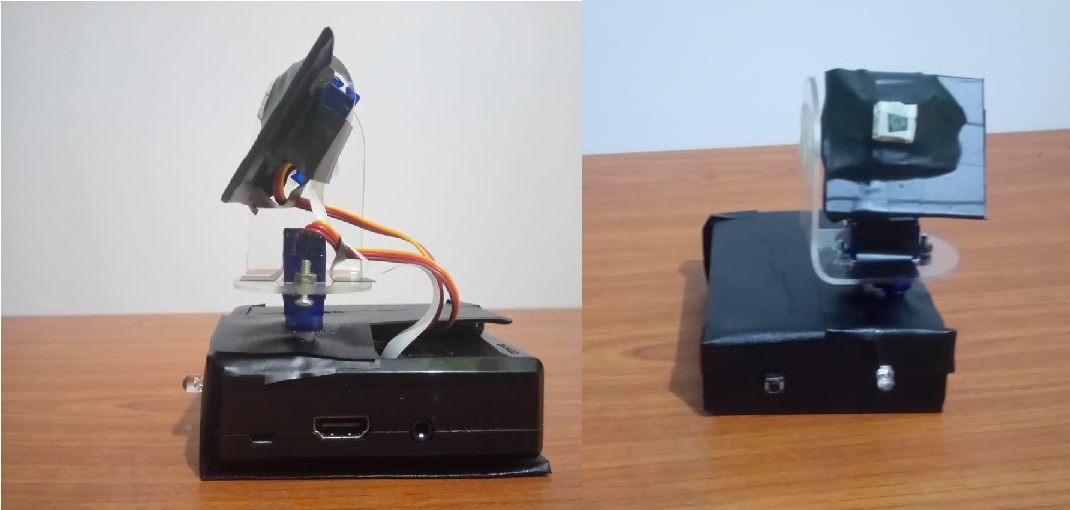
\includegraphics[scale=0.4]{device.jpg}
    \caption{Preview of the device}
    \label{fig:Preview of the final product}
\end{figure}

\subsection{Pre requisites}
The requires libraries and programs are installed by the \textbf{install.sh}. The following is the list of pre requisites, installation commands and their contribution for advanced users
%@GIHAN
\subsubsection{MQTT}
pip install paho-mqtt
\subsubsection{Python2.7}
If python3 is already installed in the system please remove it before proceeding. This can complicate things when installing python libraries.\newline

\emph{Note}: Currently opencv3 cannot be installed to python3 in raspberry pi. If it is necessary to install in python3, there is a tedious way to install opencv3 to python3 in raspberry pi 3. This is not recommended!\newline

To uninstall python3,\newline

sudo apt-get remove python3

\subsubsection{Numpy}
pip install numpy\\
This is used for faster numerical calculations.

\subsubsection{Scipy}
sudo apt-get install python-scipy\\
The pip package manager's release does not have binaries compiled to the raspberry pi architecture. apt has the working version.

\subsubsection{Opencv 3}
sudo apt-get install OpenCV-Python\\
There are numerous ways to install opencv and interface it with python. But most of them lack binaries for the raspberry pi architecture for certain algorithms. Compiling the opencv source by yourself and the apt's release works.



\subsection{FSM and Run at startup}  

When the device starts the service, initially it will be in the ready state. In this state the device will take user input through the push down button in order to start the analysis and communicate with the server. When the button is pressed, the device will go to adjust camera state where the module automatically adjust the camera angle to direct it to the infant. When the camera is rotated accordingly, the state will change to analysis. In this state a video of the infant will be recorded and analyzed. The processed information will be sent to the server for further analysis. If the analysis state needs to adjust the camera, the state will be changed and this will be repeated continuously. 

\subsection{Network setting}
The network settings are set up when the code is inserted to the node. It is explained in the section \textbf{Downloading the software}

%@GI @HARSHANA DONT WE NEED WAP CONFIG STUFF HERE.. nope!!

\subsection{Reading input}
The device reads the input from the Raspberry pi camera. The camera is directly connected to the device using the camera port in the raspberry pi. To take the user input, a push down button is available to reset the device and start the service. The input from the push down button is connected to the device using GPIO pin 11. In order to remove the unnecessary bouncing effects, 300ms software de-bouncing has been applied.

\subsection{Rotating Camera}

Given different lighting condition the detection of baby by the camera becomes the most primitive task. There are two servo motors connected to the device to turn the camera and adjust the angle of the camera to direct it to the infant. These motors are powered by the raspberry pi itself. Motor shield was not used to power the motors because the angle that the motors rotate are controlled by the software itself with a safe margin. Also the motors does not absorb much power because the camera and the equipment holding the camera is lightweight and the current drown by the power bus in the raspberry pi is capable of supplying the current required for the motors.\newline
The control signal to the servo motors are sent using GPIO pins 12 and 13 in the raspberry pi 3 module. Hardware PWM is used to give the control signal through these pins because using software PWM is consuming CPU and it might not be accurate when other processes are running concurrently. Since the hardware PWM should be controlled by changing the registry values in the raspberry pi, using pure python it is difficult to adjust these parameters. therefore, a third party software \emph{pigpio-daemon} was used. This application should be running in background in order to change the hardware PWM values from python. This can be accomplished by connecting to a port that is used to communicate with the application and sending required commands through that port.




\subsection{Pin Mapping}

Apart from the pins mentioned above, GPIO pin 21 is used to connect the LED as a output to the user to identify the state in which the device is in.

\begin{figure}[H]
    \centering
    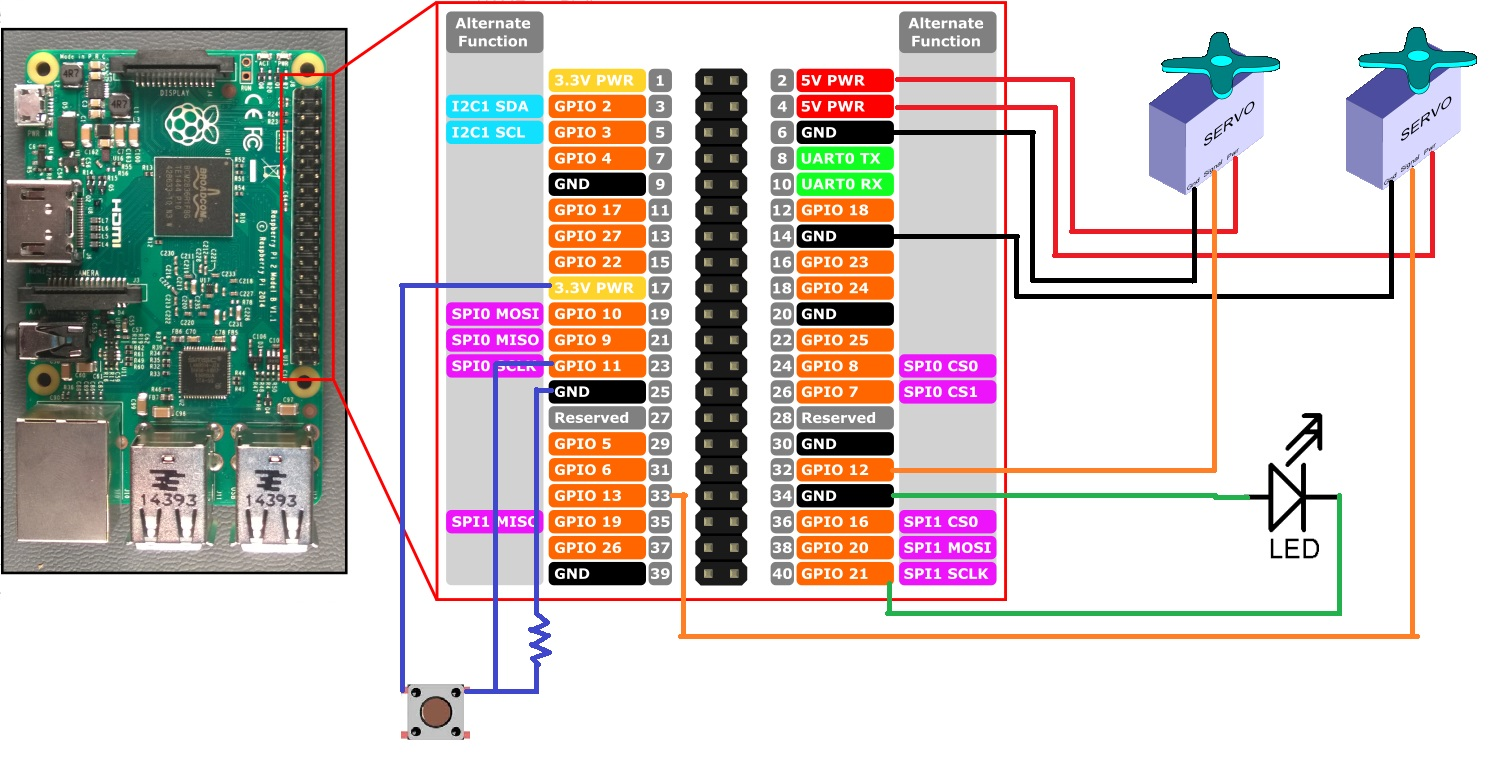
\includegraphics[scale=0.3]{pinmapping.jpg}
    \caption{Pin mapping of the Raspberry pi}
    \label{fig:Pin mapping of the Raspberry pi}
\end{figure}

\subsection{Detecting the breathing pattern}
\subsubsection{Operation}
This part of the program,
\begin{itemize}
    \item detects the breathing pattern
    \item analyzes it
    \item writes it to a detailed pdf report on the device
    \item transmits the results to the server
\end{itemize}
\subsubsection{Code}
The code for this algorithm is present at\\*
\textbf{https://github.com/TeambiteCode/Sleep\_Apnea\_Detection/tree/master/Algos}.\\
Following is a detailed description for someone who wants to implement the algorithm themselves in a different language etc:.\\

\subsubsection{Detailed algorithm}
The algorithm we propose have several steps.
\begin{itemize}
    \item The video is taken in as an array of 8 bit unsigned integers.\\
    \begin{figure}[H]
        \centering
        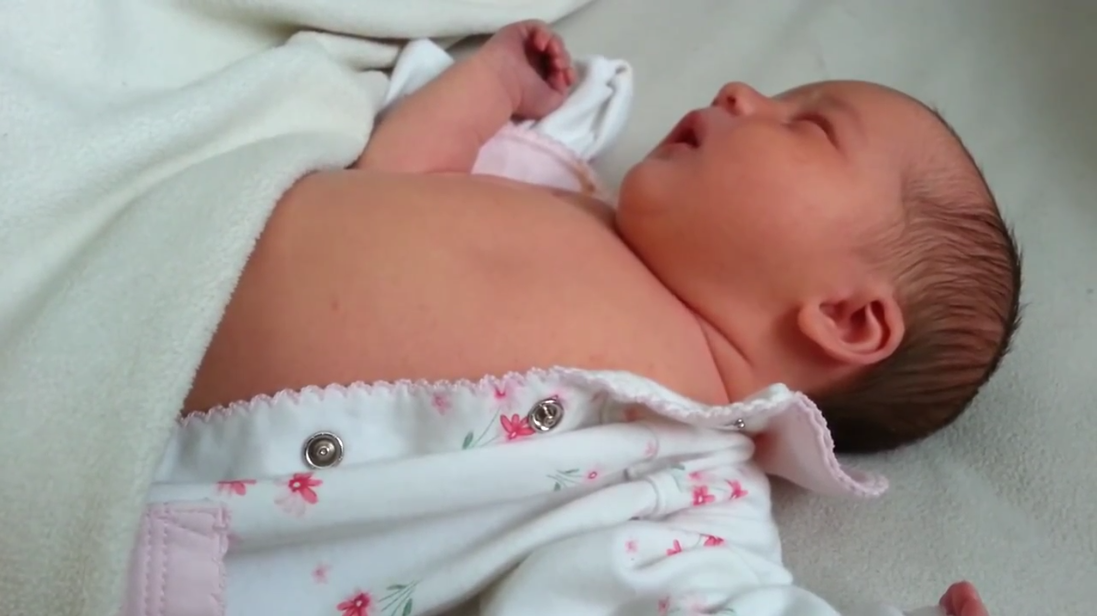
\includegraphics[keepaspectratio,scale=0.25]{video01.png}
        \caption{The original video}
        \label{fig:my_label}
    \end{figure}
    
    \item The video is fed to the \textbf{Canny edge detection algorithm}\\
    The opencv implementation of this algorithm is used. The result is a black and white video stream on where the white corresponds to the edges and black to the rest.\\
    $$E_{(t)}_{H\times W} \textrm{ is the edge matrix.}$$ 
    $$E_{(t,x,y)}=  \left \{ \begin{array}{l}
        1 \textrm{ if } E_{(t,x,y)} \textrm{ is an edge. }\\
        0 \textrm{ if } E_{(t,x,y)} \textrm{ is not an edge. }\\ 
        \end{array} \right \} $$

    \begin{figure}[H]
        \centering
        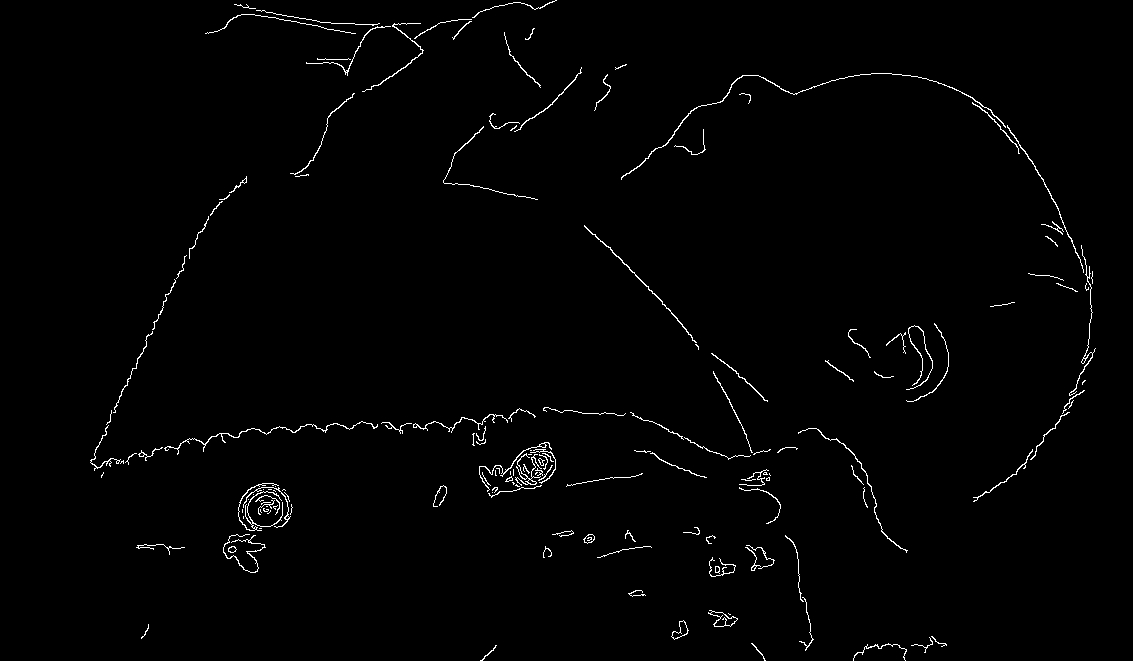
\includegraphics[keepaspectratio,scale=0.22]{video02.png}
        \caption{The edges of the video}
        \label{fig:my_label}
    \end{figure}
    
    
    \item The region of interest $A_0$ is chosen.\\
    $(x,y) \in A_0 \\x\in [ x_{0},x_{1} ] , y\in [ y_{0},y_{1} ]$\\
    As of now our algorithm requires a manual input for this region.\\We hope to automate this parameter during the time from 3rd phase evaluation to the final evaluation.\\
    
    \begin{figure}[H]
        \centering
        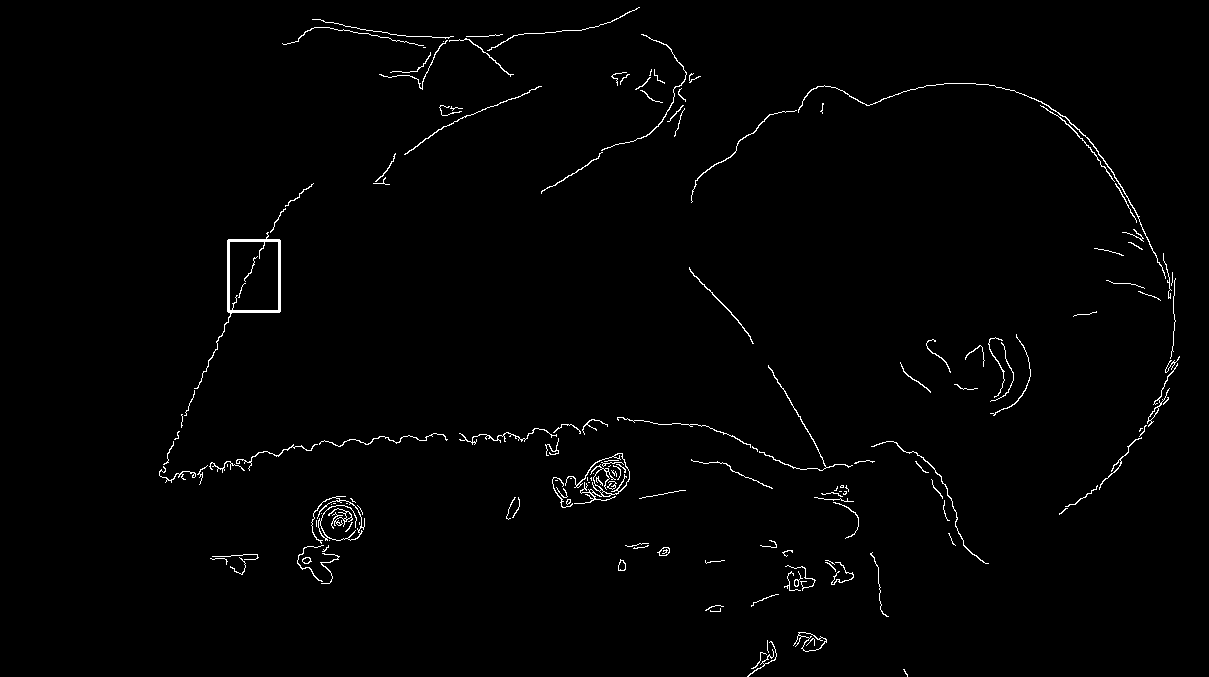
\includegraphics[keepaspectratio,scale=0.25]{video03.png}
        \caption{The region of interest}
        \label{fig:my_label}
    \end{figure}
    
    \item The centroid $C_{0}(t)$ of the edges in $A_0$ is calculated for every $t$\\
    $C_0(t)=(x_{c_0(t)},y_{c_0(t)}))$\\
    $$x_{c_0(t)} =\frac{ \sum _{(x,y) \in A} E(t,x,y) \times x}{ \sum _{(x,y) \in A} E(t,x,y)}$$\\
    $$y_{c_0(t)} =\frac{ \sum _{(x,y) \in A} E(t,x,y) \times y}{ \sum _{(x,y) \in A} E(t,x,y)}$$\\
    Special case:\\
    $(x_{c_0(t)},y_{c_0(t)})=(\frac{x_0 + x_1}{2},\frac{y_0 + y_1}{2})$ when $$\sum _{(x,y) \in A} E(t,x,y)  =0$$\\
    
    \item Then the velocity of the centroid $\underline{v}_{(t)}$ is calculated by,\\
    $\underline{v}_{(t)} =(x_{c_0(t)}-x_{c_0(t-1)})\underline{i} + (y_{c_0(t)}-y_{c_0(t-1)})\underline{j} $
    
    \item The direction along which the velocity of the centroid  $\underline{v}_{(t)}$ lie is calculated using the \textbf{Principle component analysis} as follows,\\
    Write $v_{(t)}$ as a row vector $$v_{(t)} = \left ( \begin{tabular}{c c}
         \underline{v}_{(t)} . \underline{i} & \underline{v}_{(t)} . \underline{j}\\
    \end{tabular} \right )$$
    $$v_{(t)} = \left ( \begin{tabular}{c c}
         v_{x(t)} & v_{y(t)} \\
    \end{tabular} \right )$$\\
    
    Make a matrix by taking 10 such readings and arranging them as rows,
    $$V_{(t)} = \left ( \begin{tabular}{c c}
         v_{x(t)} & v_{y(t)} \\
         v_{x(t-1)} & v_{y(t-1)} \\
         v_{x(t-2)} & v_{y(t-2)} \\....&...\\...&.....\\
         v_{x(t-9)} & v_{y(t-9)} \\
    \end{tabular} \right )\\$$
    
    Find the mean of these rows,\\
    $$\overline{v_{x(t)}}=\frac{1}{10} \sum _{i=0}^{9} v_{x(t-i)}$$
    $$\overline{v_{y(t)}}=\frac{1}{10} \sum _{i=0}^{9} v_{y(t-i)}$$
    
    Then find the difference matrix,
    
    $$D_{(t)} = V_{(t)}-\overline{V_{(t)}} = \left ( \begin{tabular}{c c}
         v_{x(t)}-\overline{v_{x(t)}} & v_{y(t)}-\overline{v_{y(t)}} \\
         v_{x(t-1)}-\overline{v_{x(t)}} & v_{y(t-1)}-\overline{v_{y(t)}} \\
         v_{x(t-2)}-\overline{v_{x(t)}} & v_{y(t-2)}-\overline{v_{y(t)}} \\....&...\\...&.....\\
         v_{x(t-9)}-\overline{v_{x(t)}} & v_{y(t-9)}-\overline{v_{y(t)}} \\
    \end{tabular} \right )$$
    
    The covariance matrix $C_{(t)}$ is calculated by,\\
    $$C_{(t)}=D_{(t)}^T .D_{(t)} $$
    
    $C_{(t)}$ is decomposed into\\
    $C_{(t)} = P_{(t)} D_{(t)} P_{(t)}^{-1}$ using eigen value decomposition.\\
    $$P_{(t)} = \left ( \begin{tabular}{cc}
         w_{1x(t)}&w_{2x(t)}  \\
         w_{1y(t)}& w_{2y(t)}
    \end{tabular}\right )$$
    and
    $$D_{(t)} = \left ( \begin{tabular}{cc}
         \lambda_{1(t)}&0  \\
         0& \lambda_{2(t)}
    \end{tabular}\right )$$
    
    Here the $P_{(t)}$ has the eigen vectors,\\
    $$\underline{w}_{1(t)}=w_{1x(t)}\underline{i}+w_{1y(t)}\underline{j}$$
    $$\underline{w}_{2(t)}=w_{2x(t)}\underline{i}+w_{2y(t)}\underline{j}$$
    
    $D_{(t)}$ has their corresponding eigen values $\lambda_{1(t)}$ and $\lambda_{2(t)}$\\
    
    The bigger value of $\lambda_{1(t)}$ and $\lambda_{2(t)}$ is chosen (let it be $\lambda_{1(t)}$ ) and the corresponsing eigen vector $\underline{w}_{1(t)}$ gives the direction of the breathing.\\
    
    The unit vector along this direction is calculated for the next steps,\\
    $$u{(t)}=\frac{\underline{w}_{1(t)}}{\|{\underline{w}_{1(t)}}\|}$$
    
    \item Now we have $\underline{u}{(t)}$ and $\underline{v}_{(t)}$. Projecting the velocity vector in the unit vector of direction gives a scalar parameter $s_{0(t)}$ that can be used to determine breathing.
    
    $$s_{0(t)}=\underline{u}{(t)} . \underline{v}_{(t)}$$
    
    \begin{figure}[H]
        \centering
        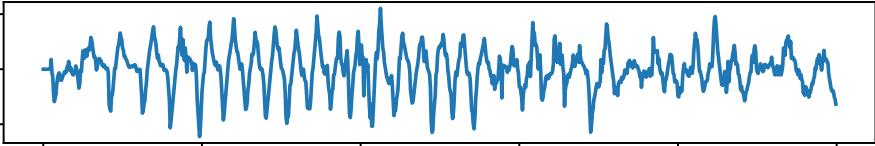
\includegraphics[width=8cm, height=3cm]{s0.png}
        \caption{$s_{0(t)}$}
        \label{fig:my_label}
    \end{figure}\\
    
    \item $s_{(0)t}$ undergoes two smoothing techniques to give,
    $$s_{1(t)} \leftarrow \textrm{ adaptive filtered } s_{0(t)} $$
    $$s_{2(t)} \leftarrow \textrm{ gaussian blurred } s_{1(t)} $$
    
    $$s_{1(t)}=s_{0(t)}\times 0.8 + s_{0(t-1)}\times0.2 $$
    Gaussian blurring is done with $15\sigma$ radius.\\
    
    \item The graph $s_{2(t)} \textrm{ - } t $ looks as follows,\\
    
    \item The peaks are found using the technique,
    \begin{center} $s_{2(t)}>s_{2(t-1)} \textrm{ and } s_{2(t)} \leq s_{2(t+1)} \Rightarrow s_{2(t)} $ is a peak.\end{center}\\
    The peaks are marked as following.\\
    
    \begin{figure}[H]
        \centering
        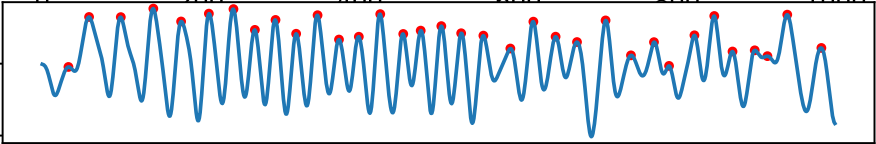
\includegraphics[width=8cm, height=3cm]{s1}
        \caption{$s_{2(t)}$ with peaks marked}
        \label{fig:my_label}
    \end{figure}\\
   
    \item The breathing intervals are calculated as the time between two peaks.
    


    

    \begin{table}[H]
    \begin{center}\begin{tabular}{|c|c|}
        \hline
         Breath number& Time for cycle / (ms) \\
         \hline
         1&1200\\2&1230\\3&1050\\4&1050\\
         ...&...\\...&...\\...&...\\...&...\\
         \hline
    \end{tabular}
        \caption{Breathing time interval report}
        \label{tab:my_label}
    \end{center}
    \end{table}    

    
    
    
\end{itemize}




\subsection{Communication}

The system uses MQTT protocol to communicate.\\*
This was implemented using paho-MQTT library by eclipse.\\*
The client publishes to 3 subtopics under the main topic : \textit{user\_name/device\_ID}. The three subtopics are : 

\begin{itemize}
    \item Data \\*
    The device publishes the actual data to this topic. The data is sent as a json message with two parameters : Timestamp, Array of data. The timestamp helps in identifying duplicates and ordering. The array of data is used to plot the graph
    \item Connection \\*
    This is the last will topic of a device. When a device disconnects (expected or unexpected manner) the broker identifies this and publishes a disconnect message to the topic. Therefore when the device connects it publishes 1 to this topic to denote that it is active and when it disconnects, the broker publishes 0 to this topic to denote that it is inactive (This is used in the Web interface).
    \item Alert \\*
    The algorithm provides timely alerts when there is a possibility of sleep apnea. The device publishes to this topics in case such an alert occurs. (This feature has been disabled due to the high number of false positives. To enable please change the flag in config.in to true).

\end{itemize}

\subsection{Security}

The communication between Node and the Broker was secured using multiple techniques. All these features are provided by paho-MQTT library. The security features are actually implemented in the Broker but the device must be configured to use them. Read the security section under broker for further details.

\begin{itemize}     
    \item Authenticate\\* Each device has device ID and access token. By combining the device ID with the user name each device would have a unique ID (Different user could have device with same device ID therefore user name and device ID are combined). The combined ID acts as the MQTT user name and the access token acts as the password. These two are used to authenticate the device. \\*The MQTT user name and password are stored in the config.ini file and is read using \textit{read} function in the \textit{configparser} library. \\*Then the user name and password can be set using \textit{username\_pw\_set} function in the MQTT library.
    \item Access Control\\* Each device has a particular topic to which it could publish. The device doesn't have permission to publish to any other topics unless the device ID and the access token are changed. The topic to which the device can publish is: \textit{user\_name/device\_ID} and the device can publish to any subtopic under it.
    \item Encryption\\* The communication uses TLS encryption to communicate with the Broker. Since the authentication send the password this is a must. It also ensures confidential transmission of data.\\*No application level encryption is used since the MQTT model uses multiple subscriber publisher model and this would make key exchange mush more complicated. Multiple subscribers imply that all the clients would need to know the key which makes it impractical.\\* TLS certificate was obtained from the broker and can be set using \textit{tls\_set} function in the MQTT library.
\end{itemize}

\subsection{Testing} %@gihan write this nicely.

Each segmant was initialy tested as a seperate unit and finaly they were connected together and tested. The information regarding the tests are as follows:

\subsubsection{Camera Alignment}


\begin{enumerate}
    \item First, the functionality of the camera is tested. Video feed taken using the camera was communicated to a computer using a communication protocol and the received video was displayed in computer screen. The color, sharpness, intensity of the camera module was tested in order to configure correct parameters.
    \item Localization of the abdomen of the infant was tested using prerecorded videos. They were analyzed in a computer and results were obtained from three different types of videos. Results are shown below. White mask is the predicted abdomen area, using filtering techniques and connected component analysis.
    \item The correct rotation of the camera module is tested using a picture of the infant and gently moving the image. It is verified that the camera follows the image with given configurations.
    \emph{Note}: This algorithm cannot identify sudden movements. But it won't be a problem since infants cannot move their body quickly.
    
\end{enumerate}

\begin{figure}[H]
    \centering
    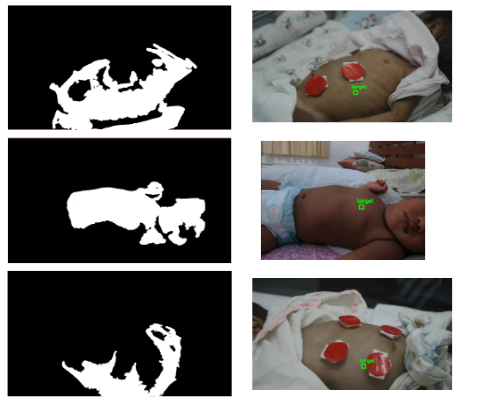
\includegraphics[scale=0.6]{b0.png}
    \caption{Baby detection algorithm}
    \label{fig:Baby detection algorithm}
\end{figure}


\clearpage
\subsubsection{Breathing pattern detection} 
\begin{itemize}
    \item Since the video data set was not labelled, the testing required labelling as well.
    \item A user friendly interface for video frame labelling was developed.
    \item The accuracy of the algorithm was tested by comparing the results of the algorithm to the human labelled data.
    \item code : https://github.com/TeambiteCode/Sleep\_Apnea\_Detection/tree/master/Testing
    \item The results of the testing were used to tune the parameters of the algorithm such as
    \begin{itemize}
        \item Radius of Gaussian filters\\
        \begin{figure}[H]
            \centering
            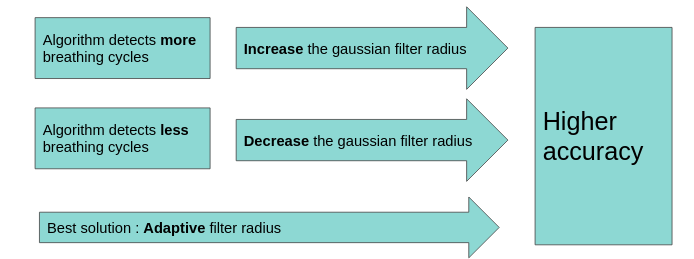
\includegraphics[scale=0.6]{unitTesting.png}
            \caption{Unit testing of the algorithm to improve accuracy}
            \label{fig:Unit testing of the algorithm to improve accuracy}
        \end{figure}
    \end{itemize}
\end{itemize}


\subsubsection{MQTT Communication} %@Suren chang subsub topic
Since Communication cannot be tested as a seperate component, it was tested together with the broker. Refer Testing Under Broker.

\subsubsection{Integration testing}
The full system has been only tested with data sets since we are still awaiting a response from the medical faculty to test the equipment.

\clearpage
\section{MQTT Broker}

MQTT plays a huge role in this system since all the real time data are send directly to the user instead of using the server. MQTT uses a publisher-subscriber mechanism (as opposed to client-server). This ensures that single client can write/listen to multiple topics while multiple clients can write/listen to the same topic. This is a form of m-n communication and, if applied in a client-server model could be slow and inefficient. To do this efficiently and in real time, MQTT was chosen. MQTT messages are much more smaller (small headers) thus offer high throughput, but cannot support larger messages. In our case this is not a problem since messages sent are small is size.\\*
Code for broker implementation can be obtained from:\\*
\textbf{https://github.com/TeambiteCode/Sleep\_Apnea\_Detection/tree/master/Mosquitto}.\\


\begin{figure}[H]
    \centering
    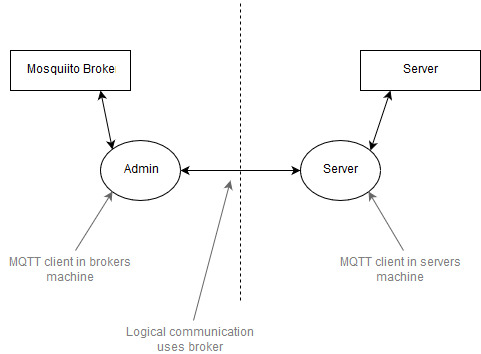
\includegraphics[scale=0.6]{ServerBroker.jpg}
    \caption{Server broker architecture}
    \label{fig:Server broker architecture}
\end{figure}


The MQTT broker was implemented independent to the server. This made testing easier, system more secure (Breach in one system would keep the other intact) and gave much more flexibility while developing specific features. This would also allow us to deploy them on different servers.\\*
Therefore the Broker must communicate with the server through a separate mechanism. In our case two MQTT clients with the following names were used:

\begin{itemize}
    \item Admin - Runs with the broker. Controls Broker
    \item Server - Runs with the client. Communicates Broker
\end{itemize}

This is the only pathway through which the broker and server communicate and transfer information. It is used when signing in or registering new device.The \textit{Server} publishes to the Admin topic to which the \textit{Admin} listens and the \textit{Admin} publishes to the server topic to which the \textit{Server} listens. Since this is a one to one communication it uses AES algorithm to encrypt the data.\\*

The implementation of MQTT client \textit{Admin} is explained in this section and the implementation of MQTT client \textit{Server} is explained in the next section\\*

\subsection{Mosquitto}

Mosquitto is used as the MQTT Broker. It can be installed as follows:\\*

\hspace*{2cm}sudo apt-get install mosquitto\\*

The MQTT broker listens to 3 ports :
\begin{itemize}
    \item 1883 (MQTT without TLS)
    \item 8883 (MQTT with TLS)
    \item 9001 (Websocket)
\end{itemize}

The listeners can be opened using \textit{listener} in Mosquitto config file (mosquitto.conf). The protocol of each listener must be specified. All other configuration are available in the default mosquitto config file. Configuring the security features are explained in the next section.\\

\subsection{Admin}

The admin client is much similar to the MQTT client in the device. It is a python based client created using paho-MQTT library. Only the  differences are explained in this section.\\
Code for admin implementation can be obtained from:\\*
\textbf{https://github.com/TeambiteCode/Sleep\_Apnea\_Detection/tree/master/Mosquitto/Admin}.\\

\begin{itemize}
    \item The client has a user name ("Admin") and password previously set and these are specified in static files (Static files explained under security/authentication).
    \item The admin is subscribed to the topic #. This is the global wild card and as a result the admin gets all the messages. Since admin is a superuser it has access to all the topics. Thus the Admin can communicate with both the server and the devices.\\*The subscription to this particular topics can be done using the \textit{subscribe} function in the MQTT library. The admin publishes to the \textit{Server} topic. This is done using the publish function.
    \item Admin controls the MySQL database used by Broker and connection to this is made using MySQLdb connector library for python.
    \item In addition to TLS protection the admin uses application level encryption. To implement this, AES algorithm and Diffie-Hellman Key Exchange protocol is used. (Explained under security). Authentication and acl are also explained in security.\\*

\end{itemize}

The \textit{Admin} MQTT-client provides the following functionality.

\subsubsection{Register Device}
When a device is registered the \textit{Server} MQTT client sends a message to this topic with the user name and password (encrypted). Admin decrypts it and then hashes the password before adding it into the user table.

\subsubsection{User login}
All real time updates are sent directly from the MQTT broker (Not the server) thus the user needs access to these topics. When a user logs in \textit{Server} (MQTT client) authenticates the user and  sends a message to this topic with the user name and password (encrypted). Admin adds a temporary entry in the user table with the user name and creates a temporary access token for the user. Then in the acls table the \textit{Admin} gives access to these topics to the user.\\

Then every time the Server requests for a config.js file, it checks database and creates a config.js file with the user name, password, topic, host, port, etc. and send it to the \textit{Server} (MQTT Client) by publishing it to the topic "Server" .When the server requests the config file, if the user name is not present in the table it doesn't add a new entry but instead sends the config.js file with no user name, thus the client would get a 404 error.\\*
The admin ensures that these entries are temporary using 4 flags:
\begin{enumerate}
    \item last will - When a client disconnects a message is posted to the \textit{disconnect} topic by the broker. This is the last will topic. The admin listens to this and removes the entry when the user disconnects. Disconnection occurs if user logs out or closes tab.
    \item keep-alive - When the client swiches from onee page to another the connection closes, but the entry should not be deleted (since he is still logged in). In this case a 300s keep-alive condition is configured in client so the broker doesn't publish to last will topic even if the client disconnects. Once the client reconnects the broker identifies this and keeps the connection alive.
    \item persistence\_limit- If the temporary entry exists indefinitely it is dangerous. Thus a persistence limit of 1hr is configured. The broker disconnects the connection after this time period and posts to the last will topic. The admin deletes the entry. The client tries to reconnect when disconnected and as a result a new connection with the broker is made using a new temporary entry.
    \item QOS - During the disconnection some information would be lost. In order to avoid this, a QOS of 1 is set for each client. As a result the broker would store the last message to each topic and when a new user connects it would send that message.
\end{enumerate}

\subsection{Security}
The broker implements security at multiple levels. At the network level a firewall is used. At transport level it uses TLS encryption. Apart from this authentication and access control in done using auth plugin by jpmens. Communication between broker and server is done using a MQTT client at each end and the communication between these 2 clients are encrypted using AES. Diffie-Hellman Key Exchange protocol is used for key exchange. Since sensitive information such as passwords are interchanged this encryption is a must.

\begin{itemize}
    \item Firewall \\* 
    The firewall blocks all other ports except for 1883 (MQTT without TLS) 8883 (MQTT with TLS) and 9001 (Websocket). Firewall was implemented using ufw (Uncomplicated Firewall) in linux (Mosquitto runs on Linux).\\*
    Firewall can be enabled using \textit{ufw enable} command\\*
    All incoming and outgoing traffic could be blocked using \textit{ufw default deny incoming} and \textit{ufw default deny outgoing} commands\\*
    The particular ports were allowed using \textit{ufw allow <port\_no>} command.
    \item Authenticate\\* 
    Authentication is done using mosquitto auth plugin with MySQL backend.\\*
    \begin{enumerate}
        \item Mosquitto auth plugin can be obtained from github,
        \item Open config.mk and change both \textit{files} and \textit{mysql} to yes and then make
        \item Next open a blank text file and add the static user name and passwords (In our case the admin client and server client\\*
        \hspace*{2cm}admin : admin\\*
        \hspace*{2cm}server : server\\*
        \item Convert to password file using following command: \\*
        \hspace*{2cm}mosquitto\_passwd - c filename\\*
        \item Include this in the mosquitto.conf file using auth\_opt\_password\_file option.
        \item Create a database in mysql with table "\textit{users}" with columns "\textit{id}" "\textit{username}", "\textit{password}" and "\textit{super}". Each time a device is registered, the username and hashed password would be added to this database by \textit{Admin} MQTT client. Each time a user logs in, \textit{Admin} does the same thing.
        \item Finally open mosquitto.conf file and include the auth plugin. This includes setting the auth\_plugin, auth\_opt\_backend, host, port, user, pass, etc.
    \end{enumerate}

    \item Access Control\\* 
    Access control is done in a hierarchical manner:
    
    \begin{figure}[H]
        \centering
        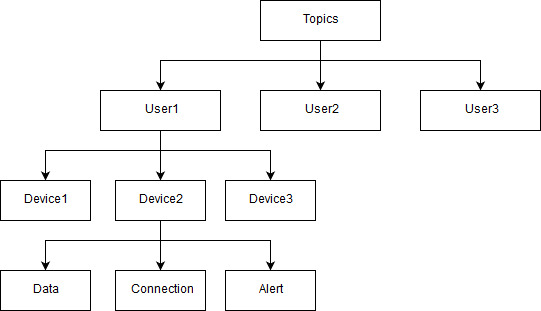
\includegraphics[scale=0.6]{ACL.jpg}
        \caption{ACL}
        \label{fig:ACL}
    \end{figure}

    A user has read access to all the device topics, but the device has read & write access to only its device topic as shown in the diagram.\\*

    ACL is aslo implemented using mosquitto auth plugin.\\*

    \begin{enumerate}
        \item Open the same database in MySQL as in authentication and create a new table "\textit{acls}" with columns "\textit{id}", "\textit{username}", "\textit{topic}" and "\textit{rw}". Each time a new device is created \textit{admin} (MQTT client) adds it to acl with the corresponding topic. Each time a user logs in \textit{admin} adds a temporary entry.
        \item Since the configuration in the conf file has been done in the previous step no need to repeat.
    \end{enumerate}

    \item Encryption\\* The communication uses TLS encryption to communicate with the devices and users. It was done using the following steps.
    \begin{enumerate}
        \item A new certificate was created as follows:\\*
        \hspace*{1cm}openssl genrsa -out server.key 2048\\*
        \hspace*{1cm}openssl req -new -out server.csr -key server.key\\*
        \item The certifice was self singed (It can be signed using a CA as well) as follows:\\*
        \hspace*{1cm}openssl genrsa -des3 -out ca.key 2048\\*
        \hspace*{1cm}openssl req -new -x509 -days 1826 -key ca.key -out ca.crt\\*
        \hspace*{1cm}openssl x509 -req -in server.csr -CA ca.crt -CAkey ca.key -CAcreateserial -out server.crt -days 360\\*
        
        \item The generated certificate was added to the broker and the mosquitto.conf file was configured to include it.
        
        \item The public certificate was added to the device.

    \end{enumerate}
    
    Apart from this the communication between Admin and Client uses AES encryption and DH key exchange. AES encyption is implemented using cryptodome package and DK key exchange is implemented using pyDH package. Both these packages can be installed using pip. The steps are as follows:

    \begin{enumerate}
        \item Install necessary packages as follows.\\
        \hspace*{1cm}pip install cryptodome\\*
        \hspace*{1cm}pip install pyDH
        \item The key exchange is done using \textit{DiffieHellman()} and \textit{gen\_public\_key()} functions and the shared key is generated using \textit{gen\_shared\_key()} function in the pyDH library. 
        \item Now that we have the shared key, the key is converted to AES usable key using AES.new() function and the encryption and decryption are done using encrypt\_and\_digest() function and decrypt\_and\_verify() function respectively. Note that the funtion creats both the cipher text and the tag where the tag is used for verification.
    \end{enumerate}
    
\end{itemize}\\
\\
Finally the broker could be run.\\*
To start database : \\*
    \hspace*{5cm}\textit{sudo service mysql start}\\*
To start Broker : \\*
    \hspace*{5cm}\textit{mosquitto -c mosquitto.conf}

\subsection{Testing}

Code for broker testing can be obtained from:\\*
\textbf{https://github.com/TeambiteCode/Sleep\_Apnea\_Detection/tree/master/Mosquitto/Test}.\\

Mosquitto provides mosquitto\_pub and msoquitto\_sub libraries for testing purposes but these were not used since their usage is limited. Instead MQTTlens was used to test which gives much interactive way to visualize the output.\\

There are no standard tests for testing mosquitto thus, the method used was based on trial and error. Multiple test cases(python clients) were created. This included clients with different user names, passwords, topics, anonymous clients (without setting username or password). On the other hand the tests were verified by using the mosquitto log and MQTTlens.\\

The log was redirected to "stdout" by setting the log\_dest in the mosquitto.conf file. The connections, disconnections and failures were observed through the log. This was used to verify that the user had to use the correct user name and password, and the TLS file had to be specified if connecting to specific port. Anonymous users were blocked on specific ports, and all other connections to unspecified ports failed. (When wrong user name or password is given the connection is refused, so the client disconnects, but if the client tries to connect to unspecified port, the firewall blocks the connection and as a result the connection fails and an error message would be displayed on the clients side. The only successful connections were, when both the user name and password were present in the mosquitto back end database. Therefore it was confirmed that the firewall and the authentication mechanism were functional.\\

The MQTTlens was subscribed to the topic # (multilevel) wild card with the user name "admin" and password "admin". Since admin is a super user, it could listen to all the topics. The test for access control was done using this. The mosquitto log would not display even if a client tried to publish / subscribe to an unauthorized topic. But the publish/ subscribe mechanism could be checked using a super user with access to all topics. Successfully connected clients from the previous stage were used to publish and subscribe to multiple topics. While the admin received all the messages, only the authorized clients, were able to publish / subscribe to particular topics. ie: The admin only received messages published by clients with access to particular topics. Therefore it was verified that the ACL mechanism was functional as well.\\*
\clearpage
\section{Server}                
The server-side was designed using python based django and rest-framework. As of djnago initially to facilitate the production environment it comes with a light weight django server and a SQLlite database. Thus the production was initally done using django's server. Since it is a lightweight production level server in order to facilitate a better deployment value the project was later transferred to an Apache server in deployment. Since the project required a site with separate clients with critical data it became necessary to build a reliable user login and session management system. So django's default login schema which facilitated session based user login system was used. \\

Code for Server can be obtained from:\\*
\textbf{https://github.com/TeambiteCode/Sleep\_Apnea\_Detection/tree/master/Server}.\\

The functionality provided by django is explained below:\\  
\subsection{Signup}                
    For the signup part each attributes where obtained separately and were obtained and processed to validated for existence and then where assigned to django's basic authentication models. When sending passwords via a the post method to avoid the theft of then sha256 algorithm was used with 100000 iterations and the final hash was stored in the server for further authentication purposes. Rest of the data where sent in a normal manner so that it can facilitate a faster access when needed sice they are not a one time used attribute in a session. 
\subsection{Login}                
    When logging in the same strategy of obtaining the password and sending the hash to the server for further processing was used for security purposes. Once the login is facilitated relevant user was saved in the session so that the user can access the data without having to signing in every single time. 
\subsection{Register device}              
    In the model a user was allowed to hold several devices. Thus in the schema devices are created with the users as a primary key. Addition devices where facilitated by the use of two particular ways. One was via the interface. Second one was with  a json request to the rest api along with the user authentication( since a browser is not used). The devices were also responsible for the addition of data. Since we have to deal with  a million data points it made sense to break the data into easily process able chunks. Thus data points were primary keyed with  the time stamps associated with them and the respective devices. The data insertion was facilitated via a json response through the rest api thus enabling the devices to automate the process rather than someone inserting via an interface all the time. The data can also be retrieved via the time stamps facilitating a better data transportation. And both the time data and the device data were denied even the read only access for an  un authorized party.    
\subsection{Delete device}                
    The deletion of devices similar to the registering were facilitated via both the interface and json response thus giving the user the option of an automated device management if the need arises. The device related data was set to cascade on device deletion thus saving memory. Apart from them via a json response with the authentication the ability to delete data with time stamps were also used. 
\subsection{Logout}                
    Logout process was done by just removing  the user details saved in the session data. % SERIOUSLY???
    
%YO BTW EXPLAIN THE VIEWS URLS MODALS AND ALL OTHER sHIT
% AND WHATEVER ELSE YOU DID  EXPLAIN ABOUT VIEWS URLS AND MODALS
% AS IN HOW YOU IMPLEMENTED. NO NEED OF THE ACTUAL CODE


\subsection{Security}               

%Explain CSRF and XSS adn SQL injecction
    Improper implementation of the database can lead to a sql injection problem. By the use of django's default user model a default check on sql requests were made manually to prevent the improper access to the sql database. At the meanwhile a malicious user can do a Cross-Site Request Forgery (CSRF) by the use of another page to send requests on behalf of the user to obtain sensible data. So when doing the post requests a CSFR token which is a non guessable and protected by HTTP's access control random number generated by the server is added to the forms. Thus the use of this large token enabled only the right client to make requests on their behalf. And as far as password transaction via a HTTP is concerned to protect it and sha256 hashing was used as mentioned before. And for the rest api's since the data is sensible an authentication only access schema was set thus even denying the read only access to the non authenticated users.

\subsection{MQTT Client}              

As explained in the previous section a MQTT client with the user name "\textit{server}" runs on the server side. This is used to communicate with the Broker. Since the broker doesn't actually listen, the communication is done with another client in the broker side (Admin) and in turns admin does the necessary changes in broker. The Server publishes to the topic admin \textit{Server} to which the Admin listens and the Admin publishes to the topic server to which the Server is subscribed. The publish and subscribe would be referred as send and receive.\\*

For security the MQTT client uses pyDH and cryptodome. These sections were explained earlier (The implementation is the same. Refer Admin, Security in MQTT broker for implementation)\\*

"Server" MQTT client provides two functions:

\subsubsection{Register Device}
When a device is registered the broker should be notified\\*
MQTT client sends a message to Admin with the user name and password (encrypted). The publishing is not done like any previous methods (creating a client then publishing) but instead it is done using a single line helper function. The helper function (Also provided by paho-MQTT library) is a one line implementation, which is used when a single message needs to be sent or received. The implementation is as follows:\\*

single("admin", payload=client.json, qos=1,
hostname="<MQTT\_host>",\\*
\hspace*{1cm}port=8883, auth=\{'username':"Server", 'password':"server"\},\\*
\hspace*{1cm}tls = \{'ca\_certs':"<ca\_certs>\}, protocol=mqtt.MQTTv311, transport="tcp")\\*

The single function is available in the paho.mqtt.publish library.
Here the first argument admin is the topic and the payload is the encrypted username and password. Apart from this, the host and the tls will have to be specified. A message received authentication is not needed since a QOS of 1 is set (sent atleast once).

\subsubsection{User login}
When a user logs in the Django does the authentication. If successful, \textit{Server} (MQTT client) gets the user and sends a message to the Admin with the user name and password (encrypted).\\

Then every time the user requests for the config.js file, the Server (MQTT Client) sends a message to the Admin with the user name and the topic needed. Then the Server waits for the reply from the Admin. Once received, this file is sent to the user. Therefore instead of dynamically creating this at the Server, the config file is made by the broker (The way the admin handles this requests is explained in the admin section).\\*
The sending message is done using the helper function as mentioned in the previous topic. The receiving message is also done as follows.(The name of function is simple):\\*

msg = simple("server", qos=0, msg\_count=1, retained=False,\\*
\hspace*{1cm}hostname="<MQTT\_host>", port=8883,\\*
\hspace*{1cm}auth=\{'username':"Server", 'password':"server"\}, tls = \{'ca\_certs':"<ca\_certs>\},\\*
\hspace*{1cm}protocol=mqtt.MQTTv311, transport="tcp")\\*

The simple function is available in the paho.mqtt.subscribe library. Notice that retained is False. This is important to make sure that retained messages are not received. Apart from this the hostname and tls needs to be set like the previous method. Once received, this message is sent to the user.\\

These actions should be trigerred when the user requests for the config.js file. This is done by making a view for this particular URL in django and including these functions inside the view. When a config.js file is requested, the server sends a request to admin and the admin replies the config.js file which is then redirected to the user.


\subsection{Testing}                % @PUNKY

    The server is made with certain schema for models and the database. But when it came to testing we had to check about their perfection. So tests were necessary. But running a buggy test on the main database may ruin the structure and the data in it. Thus for the testing purpose a new database was formed, a copy of the original one with the test period as it's lifetime and the unit tests where done on them. First the test was done for the creation of objects of the database model. Then the url mappings and rendering where validated along with the views that managed the mapping. When the tests where done they where done divided by their functionality rather than a whole. This unit testing mechanism helped us identify the bugs easier and faster. 


\section{Web Interface}

The Web interface plays a huge part, since most of the dynamic contents are generated at the users machine using MQTT client rather than enforcing it from the server. Therefore the workload on the server would be reduced whereas the workload on the broker would increase.\\*
Note that the MQTT broker uses publish subscriber mechanism therefore the incremental workload is negligible.\\*
Also Note that the usage of users resources would be simillar (Server Push vs MQTT).\\*
The Web interface was developed using HTML, CSS , javascript.\\*
Apart from these the following libraries and plugins were used:
\begin{itemize}
    \item Bootstrap
    \item MetisMenu
    \item DataTables
    \item Flot
    \item Eclipse Paho JavaScript client
\end{itemize}

The web interface consist st of multiple components. Each component of the Web Interface is described below

\subsection{Navigation Bar}
The navigation bar is included in all the pages. The navigation has two section the top bar and side bar.
\begin{itemize}
    \item Top bar\\*
    The top bar provides two feature: logout and alerts. The alert is done using MQTT javascrpit client. The client obtains the config.js file from the server. It mentions the topic as <username>/+/alert (The + is a single topic wild card therefore any alerts from devices belonging to that particular user will be listened by this client). Therefore whenever the device sends an alert, the web interface displays it by adding it to the list.\\*
    The logout functionality is implemented in the server (Refer server).
    \item Side bar\\*
    The side bar is used to go to multiple pages. It uses the metis menu package which makes the menus much more interactive.
\end{itemize}

\subsection{Dashboard}
The dashboard provides alerts as to when a device is connected or removed. It uses Bootstrap alerts div, to show the alerts but the functionality is implemented using a MQTT javascript client. A request is made to the server and it returns the config.js file. It specifies two topics : <username>/+/alert and <username>/+/connection. Therefore whenever a device belonging to the particular user connects/ disconnects or whenever an alert is sent it would be notified to the user. The MQTT message is read and a alert is created and added to the dashboard list.

\subsection{Add Device}
The add device uses a form. The devices can be added using this form. The implementation is explained in the server.

\subsection{Device List}
Device list uses DataTalbe which provides a more interactive way to visualize tables. The population of the table is done in the server. Apart from this it provides a delete device functionality which is also implemented in the server.\\*
The table has a specific column known as active which is used to see if the device is active. This is done using MQTT javascript client. The client subscribes to <username>/+/connections topic. Whenever a device connects a disconnects, a message is published to this topic. Depending on the message and the device ID the active value corresponding to a device is changed to green (active) or red (inactive). (Here the "+" is a wild card for and device\_id and by splitting the topic, the 2nd part of the topic would give the device ID)

\subsection{Charts}
The charts is done through flot. This provides a way to plot real time moving charts.\\*
The data for the charts is obtained using MQTT javascript client. The client subscribes to <username>/<device\_id>/data topic. When the message is received, it pushes(enque) the data to the existing queue and plots the queue. If the queue overflows that additional length is removed (dequed).

\section{Downloading the software}

The software for the node device and the server (in case you want to run your own server without using \textbf{http://isad.teambitecode.com}) is released as opensorce code in \textbf{https://github.com/TeambiteCode/Sleep\_Apnea\_Detection}\\
The latest release as of now is v1 availiable at\\ \textbf{https://github.com/TeambiteCode/Sleep\_Apnea\_Detection/tree/master/releases/v1}. For the ease of use, tarballs of the code is released here\\
\begin{itemize}
    \item http://teambitecode.com/projects/sleep-apnea-detection-node.tar
    \item http://teambitecode.com/projects/sleep-apnea-detection-server.tar
\end{itemize}

Following are the instructions on getting, setting and running the code.\\


\section{Device}
\begin{lstlisting}[language=bash]
wget http://teambitecode.com/projects/sleep-apnea-detection/node.tar
tar -xvf node.tar
cd node
export $SDCARD=[The mount location of the SD card here]
export $WIFI=[Wifi network ssid name here]
export $WIFIUSER=[Wifi username here]
export $WIFIPASS=[Wifi password here]
sudo chmod 700 install.sh
sudo ./install.sh
\end{lstlisting}
\clearpage
\section{Server - webserver and MQTT broker}
\begin{lstlisting}[language=bash]
sudo apt-get update
sudo apt-get install apache2
sudo apt-get install mysql-server
sudo apt-get install php libapache2-mod-php php-mcrypt php-mysql
wget http://teambitecode.com/projects/sleep-apnea-detection/server.tar
tar -xvf server.tar
cd server
sudo chmod 700 install.sh
sudo ./install.sh
\end{lstlisting}
\vspace{8cm}
\LARGE \centering END


\end{document}
